\chapter{Suggestion}
In the chapter Suggestion the datasets are selected. Further, the procedure on how to set up the experiments is to be determinded.

\section{Problems of Existing Benchmarks} \label{Problems of Existing Benchmarks}
In order to find, which Neural Network architecture is better suited for anomaly detection, first, suitable datasets have to be evaluated. Most of the papers on anomaly detection test on one of the popular benchmark datasets such as the ones created by Numenta, Yahoo, NASA, or Pei's Lab. These benchmark datasets are, however, declared as flawed by Wu and Keogh \parencite{YEAR}. Wu and Keogh state that the benchmark datasets suffer at least one of the following flaws:

\begin{enumerate}
	\item \textbf{Triviality:} Surprisingly, a sizable proportion of the problems in the benchmark datasets are trivial to solve. Triviality is hereby defined as follows: An anomaly can be found with just one line of code.
	\item \textbf{Unrealistic Density:} This flaw refers to too many anomalies in the dataset or at least in a certain region, whereas in a real world dataset the anomalous data points make up a portion of just above 0 percent.   
	\item \textbf{Mislabeled Ground Truth:} The data in all of the benchmark datasets appears to be mislabeled, with both false positives and false negatives. This is significant for a number of reasons. The majority of anomaly detectors work by computing statistics for each subsequence of some length. They may, however, place their computed label at the beginning, end, or middle of the subsequence. If caution is not exercised, an algorithm may be penalized for reporting a positive just to the left or right of a labeled region.
	\item \textbf{Run-to-failure Bias:} Because many real-world systems are run-to-failure, there is often no data to the right of the last anomaly. Therefore, a naïve algorithm that labels the last point as an anomaly has a very good chance of being correct.
\end{enumerate}

In their work, Wu and Keogh, introduced the UCR Time Series Anomaly Datasets as new benchmark, that avoids the problems listed above. However, at the start of this research project the datasets were not publicly available. Because the search for a dataset, that does not suffer from the above mentioned flaws, would be too time-consuming, the decision was taken to engineer own datasets.
\newline

\section{Anomalies}
The neural networks should be presented various types of anomalies, in order to test their ability to recognize them. Foorthuis \parencite{YEAR} compiled, in an extensive literature review, a study on the different types of anomalies. The anomalies were divided into different categories, of which foremost the quantitative multivariate aggregate anomalies are relevant for this research project, especially a) to f) (see figure \ref{fig:Anomaly_types}). These types of anomalies typically occur in time series data, that is composed by sensor data. Examples of such data could be temperature measurements or Electrocardiograms.

\begin{figure}[h]
	\centering
	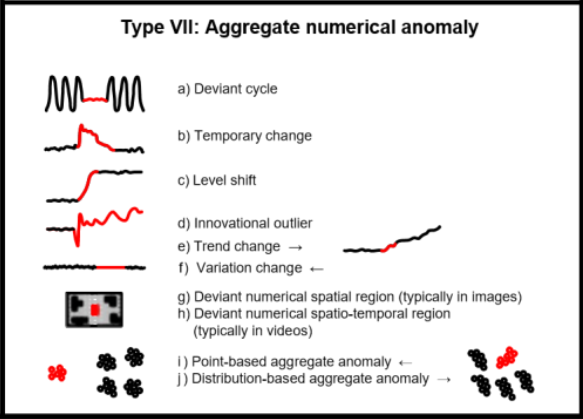
\includegraphics[scale=0.6]{Figures/series_anomaly}
	\decoRule
	\caption[Quantitative Anomalies]{Quantitative Anomalies \parencite{Foorthuis}}
	\label{fig:Anomaly_types}
    %https://arxiv.org/ftp/arxiv/papers/2007/2007.15634.pdf
\end{figure}


\section{Dataset Selection}
In the following subsections, it is proposed how and why the datasets are selected for the different experiments.

\subsection{1. Dataset}
The dataset, which should be used for the first experiment will be of synthetic nature. It consists of various cyclic patterns. In a second step, the dataset is enriched with anomalies. This way, two dataset are produced. The dataset without anomalies is used for an unsupervised learning approach whereas the dataset with labelled anomalies is used for a supervised approach. Comparing the two approaches should deliver some first insights on the abilities and learning behavior of the different neural network architectures.   

\subsection{2. Dataset}
The second dataset, which is used for anomaly detection, should consist of real data. To make sure, that the requirements mention in section \ref{Problems of Existing Benchmarks} are met, the anomalies are embedded manually into the dataset. 

\subsection{3. Dataset}
As third dataset, one of the existing benchmark datasets should be used. Despite their obvious flaws, it is still considered useful to validate the previously achieved results on an official benchmark. Further, this gives insights on the overall usefulness of the proposed neural network architectures.

\section{Design of Experiments}
Following, it is suggested how the experiments on the 3 different datasets are conducted.

\subsection{1. Experiment}
In a first experiment the learning abilities of RNN and CNN are compared. It investigated how useful the architectures are in supervised and in an unsupervised setup. 


 